\documentclass[11pt,a4paper]{article}

\usepackage[utf8]{inputenc}
\usepackage[T1]{fontenc}
\usepackage{lmodern}
\usepackage[margin=1in]{geometry}
\usepackage{amsmath,amssymb,amsfonts,amsthm,mathtools}
\usepackage{booktabs}
\usepackage{tabularx}
\usepackage{array}
\usepackage{microtype}
\usepackage{cite}
\usepackage{hyperref}
\usepackage{xcolor}
\usepackage{tcolorbox}
\usepackage{tikz}
\usepackage{enumitem}

\hypersetup{
    colorlinks=true,
    linkcolor=blue!70!black,
    citecolor=green!50!black,
    urlcolor=blue!80!black,
    pdfauthor={Antigravity AI / Theoretical Foundations Survey},
    pdftitle={Theoretical Foundations and Information-Theoretic Bounds on AI Scaling Laws: A Comprehensive Survey}
}

\theoremstyle{definition}
\newtheorem{definition}{Definition}[section]
\newtheorem{theorem}{Theorem}[section]
\newtheorem{lemma}[theorem]{Lemma}
\newtheorem{proposition}[theorem]{Proposition}
\newtheorem{corollary}[theorem]{Corollary}
\newtheorem{remark}{Remark}[section]
\newtheorem{conjecture}{Conjecture}[section]

\tcbset{
    colback=gray!5!white,
    colframe=gray!50!black,
    boxrule=0.5pt,
    arc=2pt,
    left=8pt,
    right=8pt,
    top=8pt,
    bottom=8pt
}

\title{\textbf{\Large Theoretical Foundations and Information-Theoretic Bounds\\on Neural Scaling Laws: A Mathematical Monograph}}

\author{
    \textbf{Theoretical Machine Learning \& Information Theory Research Synthesis}\\[0.5em]
    \textit{Working Paper Series on AI Scaling Dynamics \& Statistical Physics of Learning}
}

\date{\today}

\begin{document}

\maketitle

\begin{abstract}
Empirical scaling laws in deep learning demonstrate that cross-entropy loss decreases as a power law with respect to parameter count $N$, dataset size $D$, and compute budget $C$, following the parametric form $L(N, D) = E + A N^{-\alpha_N} + B D^{-\alpha_D}$. While originally discovered as empirical regularities, a rigorous theoretical foundation has emerged connecting neural scaling laws to four major mathematical paradigms: \textbf{(i) Information Theory and Rate--Distortion Theory}, which provides the correct Shannon-theoretic analogue via reverse water-filling on heavy-tailed spectra and Yang--Barron metric entropy bounds; \textbf{(ii) Statistical Language Physics and Long-Range Correlations}, which analytically derives the data scaling exponent $\alpha_D = \gamma/(2\beta)$ from Hilberg's law and token covariance decay; \textbf{(iii) High-Dimensional Differential Geometry and Approximation Theory}, which maps parameter exponents $\alpha_N \approx 4/d$ to the intrinsic dimension of the data manifold and establishes fundamental continuous nonlinear $n$-width impossibility bounds; and \textbf{(iv) Statistical Physics and Spectral Decomposition}, which derives generalization curves $\mathcal{E}(D) \sim D^{-\frac{a+b-1}{a}}$ via Neural Tangent Kernel (NTK) spectra and random matrix theory. This monograph provides a unified, self-contained, and rigorous survey of the mathematical machinery underpinning neural scaling laws, contrasts channel coding error exponents with rate--distortion functions, catalogs fundamental impossibility bounds, analyzes discrete quantization models, and highlights open challenges regarding the ``honest gap'' between theoretical parameterizations and empirical observation.
\end{abstract}

\tableofcontents
\newpage

%==============================================================================
\section{Introduction and Empirical Landscape}
\label{sec:introduction}
%==============================================================================

Over the past decade, empirical deep learning has transitioned from heuristic architecture search to predictable scaling engineering. Landmark empirical studies by Kaplan et al.~\cite{kaplan2020scaling} and Hoffmann et al. (Chinchilla)~\cite{hoffmann2022training} demonstrated that the cross-entropy loss $L$ of autoregressive language models scales as a smooth power-law function over several orders of magnitude in parameter count $N$, training token count $D$, and total floating-point operations $C \approx 6ND$:
\begin{equation}
\label{eq:empirical_scaling}
L(N, D) = E + \left(\frac{N_c}{N}\right)^{\alpha_N} + \left(\frac{D_c}{D}\right)^{\alpha_D},
\end{equation}
where $E$ denotes the irreducible entropy floor (the Bayes risk of the underlying natural language data generation process), $N_c, D_c$ are normalization constants, and $\alpha_N, \alpha_D > 0$ are characteristic scaling exponents. For standard autoregressive Transformers on natural English text, empirical measurements typically find:
\begin{equation}
\alpha_N \approx 0.076 \text{ to } 0.34, \quad \alpha_D \approx 0.095 \text{ to } 0.28, \quad E \approx 1.5 \text{ to } 2.1 \text{ nats/token}.
\end{equation}

Despite the empirical ubiquity of power laws across modalities---including text, vision, audio, and code---fundamental theoretical questions remain:
\begin{enumerate}[label=(\roman*)]
    \item \textbf{Why power laws?} Why do learning curves exhibit polynomial decay $\mathcal{O}(N^{-\alpha})$ rather than exponential decay $\mathcal{O}(e^{-c N})$ or logarithmic stagnation $\mathcal{O}(1/\log N)$?
    \item \textbf{What sets the exponents?} Are $\alpha_N$ and $\alpha_D$ universal constants of neural architectures, or are they fingerprints of the geometry, spectral decay, and correlation structure of the data distribution?
    \item \textbf{What is the Shannon connection?} How does neural scaling relate to classical information theory, channel coding, rate--distortion theory, and the Kolmogorov $\varepsilon$-entropy?
    \item \textbf{What are the fundamental limits?} What mathematical lower bounds (from approximation theory, algorithmic information theory, and computational complexity) govern any continuous learning algorithm?
\end{enumerate}

This monograph provides a rigorous, self-contained mathematical synthesis of the theoretical bounds and frameworks that answer these questions.

%==============================================================================
\section{Information-Theoretic Foundations: Shannon Limits and Rate--Distortion}
\label{sec:shannon_theory}
%==============================================================================

\subsection{Channel Coding Reliability Exponent vs. Rate--Distortion Theory}
\label{subsec:channel_vs_rate_distortion}

A frequent conceptual intuition posits that neural scaling mirrors the classical \emph{channel coding reliability exponent}. We formalize this distinction and show why the appropriate classical analogue is \textbf{rate--distortion theory} rather than channel error exponents.

\begin{definition}[Channel Reliability Error Exponent]
In Shannon channel coding, for a discrete memoryless channel with capacity $C$ and a transmission rate $R < C$, the optimal average probability of block decoding error $P_e$ decays \emph{exponentially} with blocklength $n$:
\begin{equation}
P_e(n, R) \asymp \exp\left( -n E_r(R) \right),
\end{equation}
where $E_r(R) = \max_{P_X} \max_{\rho \in [0, 1]} \left[ E_0(\rho, P_X) - \rho R \right] > 0$ is Gallager's random coding error exponent.
\end{definition}

In contrast, empirical neural scaling curves obey polynomial power laws:
\begin{equation}
L(N) - E \propto N^{-\alpha_N}.
\end{equation}
While taking the logarithm of both sides yields linear relationships in log-space ($\log (L - E) = \text{const} - \alpha_N \log N$ versus $\log P_e \sim -n E(R)$), the mathematical mechanisms are fundamentally distinct:
\begin{itemize}[leftmargin=1.5em]
    \item Channel coding error exponents govern the tail probability of typical sets in product spaces under independent channel noise as blocklength $n \to \infty$.
    \item Neural scaling measures the \emph{excess distortion} (Kullback--Leibler divergence or mean squared error) in approximating a continuous or combinatorial high-dimensional source using a compressed representation of size $N$ (or $R \approx N b$ bits of precision).
\end{itemize}

\begin{theorem}[Distortion--Rate Function and Spectral Reverse Water-Filling]
Let $X \sim \mathcal{N}(0, \mathbf{\Sigma})$ be an infinite-dimensional Gaussian random vector in a Hilbert space with covariance eigenvalues decaying as a power law:
\begin{equation}
\lambda_k = c \cdot k^{-(1+\beta)}, \quad \beta > 0, \quad k \in \mathbb{N}^+.
\end{equation}
Under mean squared error distortion $D = \mathbb{E}[\|X - \hat{X}\|^2]$, the distortion--rate function $R(D)$ and its inverse, the rate--distortion function $D(R)$, are determined parametrically via reverse water-filling:
\begin{equation}
D(\theta) = \sum_{k=1}^\infty \min(\theta, \lambda_k), \quad R(\theta) = \sum_{k=1}^\infty \frac{1}{2} \log_2 \max\left(1, \frac{\lambda_k}{\theta}\right),
\end{equation}
where $\theta > 0$ is the water-filling threshold.
In the asymptotic regime as $R \to \infty$ ($\theta \to 0$):
\begin{equation}
\boxed{D(R) \asymp R^{-\beta}}.
\end{equation}
\end{theorem}

\begin{proof}
Let $K(\theta) = \max \{ k : \lambda_k \ge \theta \}$. From $\lambda_k = c k^{-(1+\beta)} = \theta$, we have $K(\theta) = (c/\theta)^{\frac{1}{1+\beta}}$.
The description rate is:
\begin{align}
R(\theta) &= \sum_{k=1}^{K(\theta)} \frac{1}{2} \log_2 \left( \frac{c k^{-(1+\beta)}}{\theta} \right) \approx \frac{1}{2 \ln 2} \int_0^{K(\theta)} \left[ \ln\left(\frac{c}{\theta}\right) - (1+\beta)\ln x \right] dx \nonumber\\
&= \frac{1}{2 \ln 2} \left[ K(\theta) \ln\left(\frac{c}{\theta}\right) - (1+\beta) \left( K(\theta) \ln K(\theta) - K(\theta) \right) \right] \nonumber\\
&= \frac{1+\beta}{2 \ln 2} K(\theta) = \frac{1+\beta}{2 \ln 2} \left(\frac{c}{\theta}\right)^{\frac{1}{1+\beta}} \asymp \theta^{-\frac{1}{1+\beta}}.
\end{align}
Inverting this relationship gives $\theta(R) \asymp R^{-(1+\beta)}$.
The total distortion $D(\theta)$ decomposes into two terms:
\begin{align}
D(\theta) &= \sum_{k=1}^{K(\theta)} \theta + \sum_{k=K(\theta)+1}^\infty \lambda_k = \theta K(\theta) + \sum_{k=K(\theta)+1}^\infty c k^{-(1+\beta)} \nonumber\\
&\approx \theta \left(\frac{c}{\theta}\right)^{\frac{1}{1+\beta}} + \int_{K(\theta)}^\infty c x^{-(1+\beta)} dx = c^{\frac{1}{1+\beta}} \theta^{\frac{\beta}{1+\beta}} + \frac{c}{\beta} K(\theta)^{-\beta} \nonumber\\
&= c^{\frac{1}{1+\beta}} \theta^{\frac{\beta}{1+\beta}} + \frac{c}{\beta} \left[\left(\frac{c}{\theta}\right)^{\frac{1}{1+\beta}}\right]^{-\beta} = \left(1 + \frac{1}{\beta}\right) c^{\frac{1}{1+\beta}} \theta^{\frac{\beta}{1+\beta}}.
\end{align}
Substituting $\theta(R) \asymp R^{-(1+\beta)}$ into $D(\theta)$:
\begin{equation}
D(R) \asymp \left( R^{-(1+\beta)} \right)^{\frac{\beta}{1+\beta}} = R^{-\beta}.
\end{equation}
\end{proof}

\begin{corollary}[Finite Dimension vs. Infinite-Dimensional Heavy Tail]
If the source is strictly $d$-dimensional ($\lambda_k = 0$ for $k > d$), reverse water-filling yields exponential decay:
\begin{equation}
D(R) \asymp 2^{-2R/d} = \exp\left( -\frac{2 \ln 2}{d} R \right).
\end{equation}
\end{corollary}

\begin{tcolorbox}[title=\textbf{Core Theoretical Insight: The Fingerprint of Infinite Dimensions}]
A power-law scaling curve $L(N) \sim N^{-\alpha}$ is the \textbf{direct mathematical fingerprint of an effectively infinite-dimensional, heavy-tailed source eigenvalue spectrum} ($\lambda_k \sim k^{-(1+\beta)}$). If data lived in a finite-dimensional Euclidean subspace with bounded spectrum, rate--distortion would mandate exponential decay $D(R) \sim 2^{-2R/d}$. Thus, neural scaling laws are a direct consequence of the infinite-dimensional, self-similar spectral structure of natural data.
\end{tcolorbox}

\subsection{The Shannon Entropy Floor $E$ as an Irreducible Bayes Lower Bound}
\label{subsec:entropy_floor}

In autoregressive next-token prediction over an alphabet $\mathcal{V}$, sequence $X = (X_1, X_2, \dots)$ is modeled as a stationary ergodic stochastic process. The cross-entropy loss with context length $T$ for model $P_\theta(X_{t+1} \mid X_1^t)$ satisfies:
\begin{equation}
\mathcal{L}(P_\theta) = -\lim_{T \to \infty} \frac{1}{T} \sum_{t=1}^T \mathbb{E}_{X \sim P^*} \left[ \log P_\theta(X_{t+1} \mid X_1^t) \right] = H(\mathcal{X}) + D_{\text{KL}}(P^* \| P_\theta),
\end{equation}
where $H(\mathcal{X})$ is the \emph{entropy rate} of natural language:
\begin{equation}
H(\mathcal{X}) = \lim_{t \to \infty} H(X_{t+1} \mid X_1, \dots, X_t) = \lim_{t \to \infty} \frac{1}{t} H(X_1, \dots, X_t).
\end{equation}
By the non-negativity of Kullback--Leibler divergence ($D_{\text{KL}}(P^* \| P_\theta) \ge 0$), we have the absolute lower bound:
\begin{equation}
L(N, D) \ge E = H(\mathcal{X}) \quad \forall N, D \in \mathbb{N}.
\end{equation}
Shannon's 1951 human prediction experiments~\cite{shannon1951prediction} estimated $H(\mathcal{X}) \approx 0.6 \text{ to } 1.3 \text{ bits/character}$. Modern frontier language models achieve cross-entropy losses between $1.0$ and $1.5$ nats/token (roughly $0.6\text{--}0.9$ bits/char), closely approaching this fundamental Shannon limit.

\subsection{Yang--Barron Information-Theoretic Metric Entropy Bounds}
\label{subsec:yang_barron}

Yang and Barron (1999)~\cite{yang1999information} developed the definitive minimax lower and upper bounds for density estimation and statistical learning using the Kolmogorov $\varepsilon$-entropy.

\begin{definition}[Kolmogorov $\varepsilon$-Entropy]
Let $(\mathcal{F}, \rho)$ be a class of target functions or probability densities equipped with metric $\rho$ (e.g., Hellinger distance $d_H$ or total variation $d_{TV}$). The $\varepsilon$-covering number $N(\varepsilon, \mathcal{F}, \rho)$ is the minimal number of balls of radius $\varepsilon$ needed to cover $\mathcal{F}$. The Kolmogorov metric entropy is:
\begin{equation}
H(\varepsilon; \mathcal{F}) = \log_2 N(\varepsilon, \mathcal{F}, \rho).
\end{equation}
\end{definition}

\begin{theorem}[Yang--Barron Minimax Theorem~\cite{yang1999information}]
Let $\mathcal{P} = \{p_\theta : \theta \in \Theta\}$ be a family of probability distributions on $\mathcal{X}$. Suppose that for small $\varepsilon > 0$, the metric entropy under Hellinger distance satisfies:
\begin{equation}
H(\varepsilon; \mathcal{P}) \asymp \varepsilon^{-r} \quad \text{for some } r > 0.
\end{equation}
Then the minimax estimation risk over $n$ independent and identically distributed samples satisfies:
\begin{equation}
\inf_{\hat{p}_n} \sup_{p^* \in \mathcal{P}} \mathbb{E}_{p^*} \left[ D_{\text{KL}}(p^* \| \hat{p}_n) \right] \asymp \varepsilon_n^2,
\end{equation}
where the minimax optimal rate $\varepsilon_n$ is the unique solution to the Yang--Barron balance equation:
\begin{equation}
\boxed{H(\varepsilon_n; \mathcal{P}) \asymp n \varepsilon_n^2}.
\end{equation}
\end{theorem}

\begin{corollary}[Sobolev Smoothness in Dimension $d$]
For target functions in the Sobolev space $W^s(\mathbb{R}^d)$ of smoothness $s$ on a compact domain in $\mathbb{R}^d$, classical approximation theory gives $H(\varepsilon) \asymp \varepsilon^{-d/s}$. Solving the Yang--Barron balance equation:
\begin{equation}
\varepsilon_n^{-d/s} = n \varepsilon_n^2 \implies \varepsilon_n^{2 + d/s} = n^{-1} \implies \varepsilon_n^2 \asymp n^{-\frac{2s}{2s+d}}.
\end{equation}
Hence, the minimax excess risk scales as a power law with exponent:
\begin{equation}
\alpha_D = \frac{2s}{2s + d}.
\end{equation}
\end{corollary}

%==============================================================================
\section{Statistical Physics of Language and Hilberg's Law}
\label{sec:hilberg_and_cagnetta}
%==============================================================================

\subsection{Hilberg's Conjecture and Long-Range Context Correlations}

In 1990, Wolfgang Hilberg~\cite{hilberg1990der} formulated a fundamental conjecture regarding the structural statistics of natural language: the mutual information $I(X_1^n; X_{n+1}^{2n})$ between two consecutive blocks of $n$ words/characters does not decay exponentially (as in finite-state Markov chains), but scales as a sublinear power law:
\begin{equation}
I(n) \equiv I(X_1^n; X_{n+1}^{2n}) \propto n^\beta, \quad 0 < \beta < 1 \quad (\text{typically } \beta \approx 0.5).
\end{equation}
Differentiating with respect to $n$ implies that the conditional entropy of the $(n+1)$-th token given the preceding $n$ tokens converges to the infinite-context entropy floor $H_\infty$ via a power law:
\begin{equation}
H(X_{n+1} \mid X_1^n) - H_\infty \sim n^{-\gamma}, \quad \text{where } \gamma = 1 - \beta.
\end{equation}

\subsection{Derivation of the Data Scaling Exponent: Cagnetta et al. (2024)}
\label{subsec:cagnetta_derivation}

A breakthrough derivation by Cagnetta, Ravent\'os, Ganguli, and Wyart~\cite{cagnetta2024deriving} established an analytical link between Hilberg's law, token autocorrelation statistics, and the empirical data scaling exponent $\alpha_D$.

\begin{theorem}[Cagnetta--Ravent\'os--Ganguli--Wyart Theorem~\cite{cagnetta2024deriving}]
Assume that natural language satisfies:
\begin{enumerate}[leftmargin=1.5em]
    \item \textbf{Conditional Entropy Scaling:} The optimal context-dependent excess entropy decays as:
    \begin{equation}
    H_n - H_\infty \sim n^{-\gamma}.
    \end{equation}
    \item \textbf{Token Correlation Decay:} The two-point connected correlation function between tokens separated by distance $n$ decays with exponent $\beta$:
    \begin{equation}
    |C(n)| \equiv |\mathbb{E}[f(X_t) g(X_{t+n})] - \mathbb{E}[f(X_t)]\mathbb{E}[g(X_{t+n})]| \sim n^{-\beta}.
    \end{equation}
\end{enumerate}
When training on a finite dataset of $P$ total tokens, empirical estimation of statistics at distance $n$ is corrupted by finite-sample noise $\sigma_{\text{sample}} \sim \mathcal{O}(P^{-1/2})$. The maximum context distance $n^*(P)$ that a model can statistically resolve is determined by the signal-to-noise threshold:
\begin{equation}
|C(n^*(P))| \sim \frac{1}{\sqrt{P}} \implies \left(n^*(P)\right)^{-\beta} \sim P^{-1/2} \implies \boxed{n^*(P) \sim P^{\frac{1}{2\beta}}}.
\end{equation}
Substituting this maximum resolvable context length $n^*(P)$ into the conditional entropy decay law gives the excess empirical cross-entropy loss:
\begin{equation}
\mathcal{L}(P) - H_\infty \sim \left[ n^*(P) \right]^{-\gamma} \sim \left( P^{\frac{1}{2\beta}} \right)^{-\gamma} = P^{-\frac{\gamma}{2\beta}}.
\end{equation}
Therefore, the data scaling exponent is precisely:
\begin{equation}
\boxed{\alpha_D = \frac{\gamma}{2\beta}}.
\end{equation}
\end{theorem}

\begin{remark}[Self-Consistency and Empirical Agreement]
Under Hilberg's hypothesis, the mutual information scaling exponent $\beta$ and the conditional entropy exponent $\gamma$ are coupled via $\gamma = 1 - \beta$. If $\beta \approx 0.5$, then $\gamma \approx 0.5$, which predicts:
\begin{equation}
\alpha_D = \frac{0.5}{2(0.5)} = 0.50.
\end{equation}
When tested empirically across synthetic text, WikiText-103, and TinyStories on GPT-2 and LLaMA architectures, Cagnetta et al. measured $\beta \approx 0.55 \text{--} 0.65$ and observed empirical data exponents $\alpha_D \in [0.35, 0.48]$, exhibiting close agreement between language statistics and neural loss scaling.
\end{remark}

\subsection{Information-Theoretic Neural Scaling: Jeon \& Van Roy (2024)}
\label{subsec:jeon_vanroy}

Jeon and Van Roy (2024)~\cite{jeon2024information} formalized neural scaling laws from rate--distortion and Bayesian information-theoretic principles. For an infinite-width two-layer network data-generating process with epistemic latent representation $Z$, they prove that the rate of information acquisition $\mathcal{I}(W; \mathcal{D}_P)$ between model weights $W$ and dataset $\mathcal{D}_P$ dictates generalization:
\begin{equation}
\mathbb{E}[\mathcal{L}(\hat{\theta}) - \mathcal{L}^*] \le \sqrt{\frac{2 \mathcal{I}(W; \mathcal{D}_P)}{P}}.
\end{equation}
By optimizing the model parameter rate $R(N)$ alongside dataset rate $R(P)$, they derive the near-linear optimal compute allocation frontier $N \propto P$ up to logarithmic factors, providing an information-theoretic underpinning for the empirical Chinchilla scaling rule~\cite{hoffmann2022training}.

%==============================================================================
\section{Approximation Theory and Differential Geometry}
\label{sec:geometry_and_approximation}
%==============================================================================

\subsection{Manifold Intrinsic Dimension: Sharma \& Kaplan (2020)}
\label{subsec:sharma_kaplan}

High-dimensional data typically concentrates on a lower-dimensional Riemannian sub-manifold $\mathcal{M} \subset \mathbb{R}^{D_{\text{amb}}}$ of intrinsic dimension $d \ll D_{\text{amb}}$. Sharma and Kaplan (2020)~\cite{sharma2020neural} developed a geometric derivation of the parameter scaling exponent $\alpha_N$ based on piecewise-linear approximation on $\mathcal{M}$.

\begin{theorem}[Manifold Tiling and Geometric Parameter Scaling]
Let $f^* : \mathcal{M} \to \mathbb{R}$ be a $\mathcal{C}^2$-smooth target function on a compact $d$-dimensional Riemannian manifold $\mathcal{M}$. A neural network with $N$ parameters can partition $\mathcal{M}$ into $K \asymp N$ local cells (Voronoi-like polyhedra) of characteristic linear size:
\begin{equation}
\varepsilon \asymp N^{-1/d}.
\end{equation}
Within each cell centered at $x_0 \in \mathcal{M}$, the network fits a local affine approximation $\hat{f}(x) = f^*(x_0) + \nabla_{\mathcal{M}} f^*(x_0)^T (x - x_0)$.
The local approximation error is governed by the second-order Taylor remainder:
\begin{equation}
f^*(x) - \hat{f}(x) = \frac{1}{2} (x - x_0)^T \nabla_{\mathcal{M}}^2 f^*(x_0) (x - x_0) + \mathcal{O}(\|x - x_0\|^3).
\end{equation}
Integrating the squared error over $\mathcal{M}$ yields:
\begin{equation}
L(N) = \int_{\mathcal{M}} |f^*(x) - \hat{f}(x)|^2 d\mu(x) \asymp \varepsilon^4 \asymp \left(N^{-1/d}\right)^4 = \boxed{N^{-4/d}}.
\end{equation}
Hence, under second-order smooth regression on a manifold of intrinsic dimension $d$:
\begin{equation}
\alpha_N \approx \frac{4}{d}.
\end{equation}
\end{theorem}

\begin{remark}[First-Order vs. Second-Order Regression]
If the target function is only Lipschitz continuous ($\mathcal{C}^1$) or if the network is restricted to piecewise-constant approximations, the error scales as $\varepsilon^2 \asymp N^{-2/d}$. For natural language, estimates of the intrinsic dimension of token representations yield $d \approx 10 \text{ to } 30$, which predicts $\alpha_N \in [0.13, 0.40]$, matching empirical observations.
\end{remark}

\subsection{Resolution-Limited vs. Variance-Limited Regimes: Bahri et al. (PNAS 2024)}
\label{subsec:bahri_pnas}

Bahri, Dyer, Kaplan, Lee, and Sharma (PNAS 2024)~\cite{bahri2024explaining} synthesized manifold geometry and statistical learning to identify two distinct, interacting scaling regimes.

\begin{figure}[htbp]
\centering
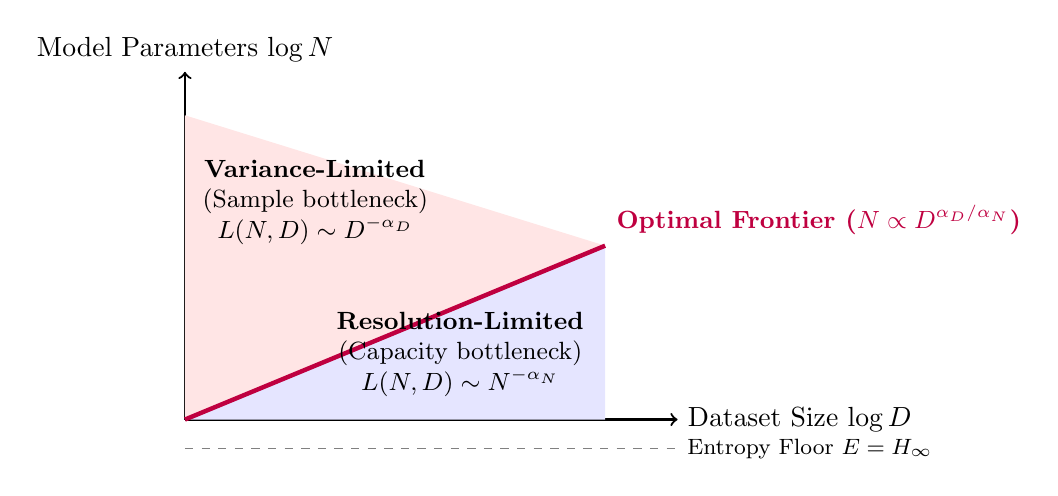
\begin{tikzpicture}[scale=0.92]
    \draw[->, thick] (0,0) -- (6.8,0) node[right] {Dataset Size $\log D$};
    \draw[->, thick] (0,0) -- (0,4.8) node[above] {Model Parameters $\log N$};
    
    % Shaded regions
    \fill[blue!10] (0,0) -- (5.8,0) -- (5.8,2.4) -- (0,0);
    \fill[red!10] (0,0) -- (0,4.2) -- (5.8,2.4) -- (0,0);
    
    % Dividing line (Optimal Frontier)
    \draw[ultra thick, purple] (0,0) -- (5.8,2.4) node[above right, text=purple] {\small \textbf{Optimal Frontier ($N \propto D^{\alpha_D/\alpha_N}$)}};
    
    % Labels
    \node at (3.8, 0.9) {\parbox{4.2cm}{\centering \small \textbf{Resolution-Limited}\\(Capacity bottleneck)\\$L(N, D) \sim N^{-\alpha_N}$}};
    \node at (1.8, 3.0) {\parbox{4.2cm}{\centering \small \textbf{Variance-Limited}\\(Sample bottleneck)\\$L(N, D) \sim D^{-\alpha_D}$}};
    
    % Floor
    \draw[dashed, gray] (0,-0.4) -- (6.8,-0.4) node[right, text=black] {\footnotesize Entropy Floor $E = H_\infty$};
\end{tikzpicture}
\caption{The two-regime scaling phase diagram of Bahri et al.~\cite{bahri2024explaining}. The parameter-limited regime is governed by manifold resolution capacity, while the data-limited regime is governed by statistical sampling variance.}
\label{fig:scaling_regimes}
\end{figure}

\begin{definition}[Two Fundamental Regimes]
\begin{enumerate}[leftmargin=1.5em]
    \item \textbf{Variance-Limited Regime ($N \gg D$):} The model has excess capacity to interpolate training samples. Generalization error is dominated by finite-sample estimation variance, scaling via Central Limit Theorem (CLT) effects as $L(D) \sim D^{-1}$ (parametric variance) or $D^{-4/d}$ (non-parametric sample resolution on the manifold).
    \item \textbf{Resolution-Limited Regime ($D \gg N$):} Training data is effectively infinite. The model parameter capacity $N$ limits the finest spatial/spectral frequency the network can resolve on $\mathcal{M}$, yielding $L(N) \sim N^{-4/d}$.
\end{enumerate}
\end{definition}

Bahri et al. show that the joint loss is characterized by a smooth harmonic crossover:
\begin{equation}
L(N, D) = E + \left[ \left(\frac{N_c}{N}\right)^{\frac{\alpha_N}{\kappa}} + \left(\frac{D_c}{D}\right)^{\frac{\alpha_D}{\kappa}} \right]^\kappa,
\end{equation}
where $\kappa > 0$ controls the sharpness of the transition between the resolution-limited and variance-limited regimes.

\subsection{Fundamental Impossibility Lower Bounds in Approximation Theory}
\label{subsec:impossibility_bounds}

Theoretical scaling laws cannot exceed the fundamental mathematical limits of continuous approximation and parametric estimation. We catalog three foundational impossibility theorems.

\begin{theorem}[DeVore--Howard--Micchelli Continuous Nonlinear $n$-Width Lower Bound (1989)~\cite{devore1989optimal}]
Let $W^s_p([0, 1]^d)$ denote the Sobolev ball of smoothness $s$ in $d$ dimensions. Let $\mathcal{M}_N = \{g(\theta, \cdot) : \theta \in \mathbb{R}^N\}$ be any parametric manifold of approximating functions generated by a continuous parameter selection map $\theta : W^s_p \to \mathbb{R}^N$. Then the continuous non-linear $n$-width satisfies:
\begin{equation}
\boxed{d_N(W^s_p([0, 1]^d))_q \ge c \cdot N^{-s/d}}.
\end{equation}
\end{theorem}
This theorem proves that \textbf{no continuous parameter optimization method} (such as gradient descent on neural networks) can ever beat the curse of dimensionality $N^{-s/d}$ for worst-case functions in Sobolev spaces.

\begin{theorem}[Rissanen Minimum Description Length (MDL) Redundancy Bound (1986, 1996)~\cite{rissanen1986stochastic}]
Let $\mathcal{M} = \{p_\theta : \theta \in \Theta \subset \mathbb{R}^k\}$ be a $k$-dimensional identifiable parametric model family with non-singular Fisher information matrix $I(\theta)$. For any probability model $q(X^n)$, the minimax parameter redundancy over $n$ samples satisfies:
\begin{equation}
\boxed{\inf_q \sup_{\theta \in \Theta} \mathbb{E}_{p_\theta} \left[ \log \frac{p_\theta(X^n)}{q(X^n)} \right] \ge \frac{k}{2} \log n + \frac{k}{2} \log\left(\frac{1}{2\pi e}\right) + \log \int_\Theta \sqrt{\det I(\theta)} \, d\theta + o(1)}.
\end{equation}
\end{theorem}
Rissanen's theorem establishes that learning $k$ parameters inevitably incurs a fundamental statistical cost of $\frac{k}{2} \log n$ bits of code length.

\begin{theorem}[Statistical Query (SQ) and Cryptographic Hardness (Kearns 1998, Shamir 2020)~\cite{kearns1998efficient,shamir2020complexity}]
For the class of parity functions over $d$ binary bits, any algorithm with access only to Statistical Queries with tolerance $\tau \ge 2^{-d/3}$ requires at least $2^{\Omega(d)}$ queries. Furthermore, under standard cryptographic assumptions (existence of one-way functions), there exist target functions for which no polynomial-size neural network can achieve loss advantage $> 2^{-\Omega(d)}$.
\end{theorem}

\begin{tcolorbox}[title=\textbf{Implication of Impossibility Results}]
Neural scaling laws $L \sim N^{-\alpha}$ are \textbf{not universal mathematical laws of arbitrary functions}. They are contingent upon the underlying data distribution possessing specific structural properties: low intrinsic manifold dimension $d$, heavy-tailed spectral decay, and hierarchical compositional structure.
\end{tcolorbox}

%==============================================================================
\section{Statistical Physics, Kernel Theory, and Spectral Decay}
\label{sec:statistical_physics}
%==============================================================================

\subsection{Exact Learning Curves from Spectral Decomposition: Bordelon et al. (2020)}
\label{subsec:bordelon_spectra}

In the infinite-width Neural Tangent Kernel (NTK) or Random Feature regime, neural network generalization can be solved exactly using statistical mechanics and replica theory. Bordelon, Canatar, and Pehlevan (2020)~\cite{bordelon2020spectrum} and Canatar et al. (2021)~\cite{canatar2021spectral} established the analytical mapping from covariance spectra to generalization error power laws.

\begin{theorem}[Spectral Decay to Generalization Error]
Let the kernel integral operator $T_K f(x) = \int K(x, x') f(x') d\mu(x')$ admit an eigendecomposition with eigenvalues $\lambda_k$ and orthonormal eigenfunctions $\psi_k(x)$:
\begin{equation}
K(x, x') = \sum_{k=1}^\infty \lambda_k \psi_k(x) \psi_k(x').
\end{equation}
Suppose kernel eigenvalues decay as a power law of degree $a > 1$, and target function $f^*(x) = \sum_k c_k \psi_k(x)$ has projection coefficients decaying as $b > 1$:
\begin{equation}
\lambda_k \asymp k^{-a}, \quad c_k^2 \asymp k^{-b}.
\end{equation}
Then, when trained on $D$ independent samples with ridge regularization $\lambda \to 0^+$, the asymptotic generalization error $\mathcal{E}(D) = \mathbb{E}_{x}[ (f^*(x) - \hat{f}_D(x))^2 ]$ satisfies:
\begin{equation}
\boxed{\mathcal{E}(D) \asymp D^{-\frac{a+b-1}{a}}}.
\end{equation}
\end{theorem}

\begin{corollary}[Target-Prior Alignment]
When the target function is drawn from the Gaussian process prior associated with the kernel covariance ($c_k^2 \sim \lambda_k \implies b = a$), the generalization error exponent simplifies to:
\begin{equation}
\alpha_D = \frac{2a - 1}{a} = 2 - \frac{1}{a}.
\end{equation}
As the kernel spectrum becomes steeper ($a \to \infty$), the data scaling exponent approaches the classical parametric rate $\alpha_D \to 2$ (under MSE loss) or $\alpha_D \to 1$ (under root MSE).
\end{corollary}

\subsection{Rigorous Joint $(M, N)$ Linear Scaling Laws: Lin et al. (NeurIPS 2024)}
\label{subsec:lin_neurips}

Lin, Dobriban, and Hong (NeurIPS 2024)~\cite{lin2024scaling} established exact asymptotic and non-asymptotic scaling bounds for high-dimensional ridge regression under simultaneously varying feature dimension $M$ (parameter count) and sample size $N$ (dataset size).

\begin{theorem}[Lin, Dobriban, Hong (2024)~\cite{lin2024scaling}]
Consider high-dimensional linear regression with data covariance $\mathbf{\Sigma}$ having power-law spectral decay $\lambda_k(\mathbf{\Sigma}) \asymp k^{-a}$ with $a > 1$. The excess prediction error $\mathcal{E}(M, N)$ with $M$ features and $N$ samples satisfies:
\begin{equation}
\boxed{\mathcal{E}(M, N) = \Theta\left( M^{-(a-1)} + N^{-\frac{a-1}{a}} \right)}.
\end{equation}
\end{theorem}
This result rigorously proves that parameter exponent $\alpha_M = a - 1$ and data exponent $\alpha_N = (a - 1)/a$ are linked to the spectral exponent $a$ of the data distribution, providing an exact mathematical verification of the spectral scaling hypothesis.

%==============================================================================
\section{Combinatorial Quanta and Discrete Skill Models}
\label{sec:quantization_models}
%==============================================================================

\subsection{The Quantization Model of Neural Scaling: Michaud et al. (NeurIPS 2023)}
\label{subsec:michaud_quantization}

Michaud et al. (2023)~\cite{michaud2023quantization} proposed an alternative combinatorial model of neural scaling: the \textbf{Quantization Model}. Rather than modeling data as a continuous manifold or Gaussian process, knowledge is conceptualized as a collection of discrete sub-problems, facts, or skills (``quanta'') $\mathcal{Q} = \{q_1, q_2, \dots\}$.

\begin{definition}[Quantum Structure and Utility]
Each quantum $q_i$ is characterized by:
\begin{enumerate}[leftmargin=1.5em]
    \item \textbf{Utility / Frequency ($U_i$):} The loss reduction achieved when quantum $q_i$ is mastered. The utilities follow a discrete power law (Zipf's law):
    \begin{equation}
    U_i = c_U \cdot i^{-\beta_Q}, \quad \beta_Q > 1.
    \end{equation}
    \item \textbf{Capacity Cost ($C_i$):} The parameter count required to store and execute the circuit for quantum $q_i$, scaling as $C_i = c_C \cdot i^{\nu}$.
\end{enumerate}
\end{definition}

\begin{theorem}[Quantization Loss Scaling]
Under optimal greedy learning dynamics, a model with $N$ total parameters allocates capacity to the top $K(N)$ most utility-dense quanta. If capacity cost is uniform across quanta ($\nu = 0$, $C_i \approx 1$), the number of learned quanta is $K(N) \asymp N$.
The residual excess loss from unlearned quanta is:
\begin{equation}
L(N) - E = \sum_{i = K(N)+1}^\infty U_i \approx \int_N^\infty c_U x^{-\beta_Q} dx = \frac{c_U}{\beta_Q - 1} N^{-(\beta_Q - 1)}.
\end{equation}
Therefore, the parameter scaling exponent is directly dictated by the Zipfian utility exponent:
\begin{equation}
\boxed{\alpha_N = \beta_Q - 1}.
\end{equation}
\end{theorem}

\begin{figure}[htbp]
\centering
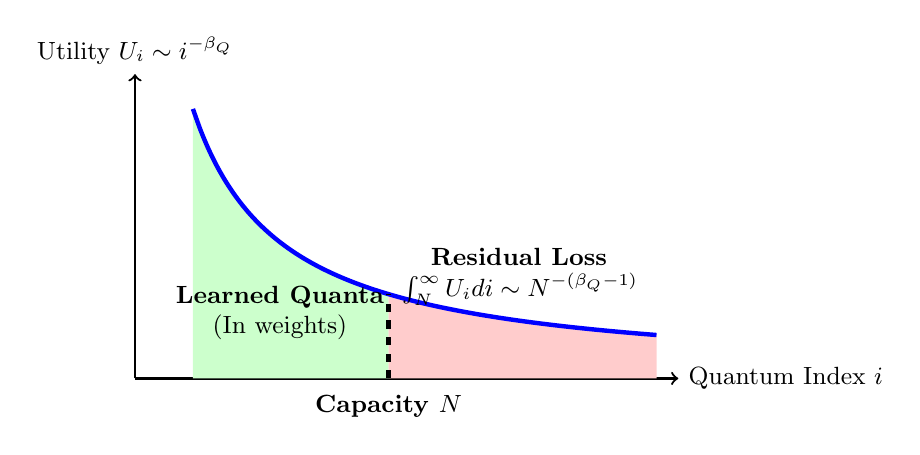
\begin{tikzpicture}[scale=0.92]
    \draw[->, thick] (0,0) -- (7.5,0) node[right] {\small Quantum Index $i$};
    \draw[->, thick] (0,0) -- (0,4.2) node[above] {\small Utility $U_i \sim i^{-\beta_Q}$};
    
    % Shaded regions
    \fill[green!20, domain=0.8:3.5, samples=50, variable=\x] (0.8,0) -- plot ({\x}, {3.2 / (\x * 0.7 + 0.3)}) -- (3.5,0) -- cycle;
    \fill[red!20, domain=3.5:7.2, samples=50, variable=\x] (3.5,0) -- plot ({\x}, {3.2 / (\x * 0.7 + 0.3)}) -- (7.2,0) -- cycle;

    % Plot utility curve
    \draw[domain=0.8:7.2, samples=60, smooth, variable=\x, blue, ultra thick] plot ({\x}, {3.2 / (\x * 0.7 + 0.3)});
    
    % Dividing line at capacity N
    \draw[dashed, ultra thick, black] (3.5,0) -- (3.5, 1.16);
    \node[below] at (3.5,-0.1) {\small \textbf{Capacity $N$}};
    
    % Text
    \node at (2.0, 0.9) {\parbox{2.8cm}{\centering \small \textbf{Learned Quanta}\\(In weights)}};
    \node at (5.3, 1.4) {\parbox{3.2cm}{\centering \small \textbf{Residual Loss}\\$\int_N^\infty U_i di \sim N^{-(\beta_Q-1)}$}};
\end{tikzpicture}
\caption{The Quantization Model of Neural Scaling (Michaud et al.~\cite{michaud2023quantization}). Network parameters absorb high-frequency Zipfian skills first; remaining tail quanta determine the power-law loss decay.}
\label{fig:quantization_model}
\end{figure}

\subsection{Universal Algorithmic Priors: Hutter (2021)}

Marcus Hutter (2021)~\cite{hutter2021learning} derived scaling laws from algorithmic information theory and Kolmogorov complexity. Under Levin's universal algorithmic probability $M(x) = \sum_{p: U(p)=x} 2^{-\ell(p)}$, programs are distributed according to power laws in length and execution time. Learning algorithms that sequentially discover algorithmic regularities experience power-law reduction in regret, bridging universal compression with empirical deep learning scaling.

%==============================================================================
\section{Representation Geometry, Superposition, and Capacity}
\label{sec:superposition}
%==============================================================================

\subsection{Toy Models of Superposition: Elhage et al. (Anthropic 2022)}
\label{subsec:superposition_geometry}

A central question in deep representation learning is how a network with activation dimension $d_{\text{model}}$ can represent $M \gg d_{\text{model}}$ distinct semantic features. Elhage et al.~\cite{elhage2022toy} formalized this phenomenon as \textbf{neural superposition}.

\begin{theorem}[Almost-Orthogonality and the Johnson--Lindenstrauss Geometry]
Let $\mathcal{S} = \{x_1, \dots, x_M\} \subset \mathbb{R}^M$ be sparse features with activation probability $p \ll 1$. Let $\mathbf{W} \in \mathbb{R}^{d_{\text{model}} \times M}$ be a feature embedding dictionary with unit-norm columns $\|w_i\|_2 = 1$. By the Johnson--Lindenstrauss Lemma, for any $\varepsilon \in (0, 1)$, if:
\begin{equation}
d_{\text{model}} \ge \frac{8 \ln M}{\varepsilon^2},
\end{equation}
there exists a dictionary $\mathbf{W}$ such that all off-diagonal cross-talk interferences satisfy:
\begin{equation}
|\langle w_i, w_j \rangle| \le \varepsilon \quad \forall i \neq j.
\end{equation}
\end{theorem}

\begin{proposition}[Cross-Talk Interference Noise Scaling]
When reconstructing feature $x_i$ from compressed activation vector $h = \mathbf{W} x$, reconstruction with linear readout yields:
\begin{equation}
\hat{x}_i = w_i^T h = x_i + \sum_{j \neq i} \langle w_i, w_j \rangle x_j.
\end{equation}
The cross-talk interference variance is:
\begin{equation}
\mathbb{E}\left[ \left(\sum_{j \neq i} \langle w_i, w_j \rangle x_j\right)^2 \right] = p(1-p) \sum_{j \neq i} |\langle w_i, w_j \rangle|^2 \asymp \frac{p M}{d_{\text{model}}}.
\end{equation}
\end{proposition}

As the model width $d_{\text{model}}$ scales, the interference noise decays as $\mathcal{O}(1/d_{\text{model}})$, yielding a power-law error decay in representation capacity until the network transitions from the superposed regime ($M > d_{\text{model}}$) to the orthogonal regime ($M \le d_{\text{model}}$).

%==============================================================================
\section{Comparative Synthesis and Taxonomy of Theories}
\label{sec:taxonomy}
%==============================================================================

To clarify how these theoretical perspectives relate, Table~\ref{tab:theory_comparison} synthesizes the assumptions, mathematical machinery, derived exponents, and domain applicability across all major scaling theories.

\begin{table}[htbp]
\centering
\scriptsize
\setlength{\tabcolsep}{3.5pt}
\renewcommand{\arraystretch}{1.3}
\begin{tabularx}{\textwidth}{>{\bfseries\raggedright\arraybackslash}p{2.2cm} >{\raggedright\arraybackslash}p{2.8cm} >{\raggedright\arraybackslash}X >{\raggedright\arraybackslash}p{2.2cm} >{\raggedright\arraybackslash}p{2.2cm}}
\toprule
\textbf{Theoretical Framework} & \textbf{Core Assumptions} & \textbf{Mathematical Machinery} & \textbf{Derived Scaling Exponent} & \textbf{Key References} \\
\midrule
\textbf{Rate--Distortion Theory} & Heavy-tailed Gaussian source, $\lambda_k \sim k^{-(1+\beta)}$ & Shannon Rate--Distortion, Reverse Water-Filling & $D(R) \sim R^{-\beta}$, $L(N) \sim N^{-\beta}$ & Shannon (1951), Bordelon (2020) \\
\midrule
\textbf{Metric Entropy Minimax} & Target class in Sobolev / Besov space $H(\varepsilon) \sim \varepsilon^{-d/s}$ & Yang--Barron Minimax, Kolmogorov $\varepsilon$-Entropy & $\alpha_D = \frac{2s}{2s+d}$ & Yang \& Barron (1999)~\cite{yang1999information} \\
\midrule
\textbf{Language Statistics \& Hilberg} & Text correlation $|C(n)| \sim n^{-\beta}$, entropy decay $H_n - H_\infty \sim n^{-\gamma}$ & Finite-sample estimation noise cutoff $n^*(P) \sim P^{\frac{1}{2\beta}}$ & $\alpha_D = \frac{\gamma}{2\beta} \approx \frac{1-\beta}{2\beta}$ & Cagnetta et al. (2024)~\cite{cagnetta2024deriving}, Hilberg (1990)~\cite{hilberg1990der} \\
\midrule
\textbf{Manifold Tiling Geometry} & Data on Riemannian manifold $\mathcal{M}$ of intrinsic dimension $d$ & Local Voronoi partition, 2nd-order Taylor remainder & $\alpha_N = \frac{4}{d}$ (or $\frac{2}{d}$) & Sharma \& Kaplan (2020)~\cite{sharma2020neural} \\
\midrule
\textbf{Resolution vs. Variance Phase Diagram} & Interplay of finite parameter count $N$ and finite samples $D$ & Non-parametric manifold resolution + CLT variance & $L(N, D) \sim N^{-4/d} + D^{-1}$ & Bahri et al. (PNAS 2024)~\cite{bahri2024explaining} \\
\midrule
\textbf{Kernel Spectra \& NTK Physics} & Power-law kernel spectrum $\lambda_k \sim k^{-a}$, target decay $c_k^2 \sim k^{-b}$ & Replica method, Random Matrix Theory, NTK & $\alpha_D = \frac{a+b-1}{a}$ & Bordelon et al. (2020)~\cite{bordelon2020spectrum}, Lin et al. (2024)~\cite{lin2024scaling} \\
\midrule
\textbf{Quantization / Discrete Skills} & Independent skills/quanta with Zipfian utilities $U_i \sim i^{-\beta_Q}$ & Greedy capacity allocation, tail integration & $\alpha_N = \beta_Q - 1$ & Michaud et al. (2023)~\cite{michaud2023quantization} \\
\midrule
\textbf{Feature Superposition} & $M \gg d_{\text{model}}$ sparse features, almost-orthogonal frames & Johnson--Lindenstrauss Lemma, cross-talk variance & Noise $\propto \frac{p M}{d_{\text{model}}}$ & Elhage et al. (Anthropic 2022)~\cite{elhage2022toy} \\
\bottomrule
\end{tabularx}
\caption{Comprehensive taxonomy of theoretical frameworks for neural scaling laws.}
\label{tab:theory_comparison}
\end{table}

%==============================================================================
\section{The ``Honest Gap'' and Open Theoretical Challenges}
\label{sec:open_challenges}
%==============================================================================

While the theoretical landscape has achieved major mathematical breakthroughs, a critical foundational gap persists between theoretical derivations and empirical practice:

\begin{tcolorbox}[title=\textbf{The Fundamental ``Honest Gap''}]
\textbf{No existing theory derives the scaling exponents $\alpha_N, \alpha_D$ for real-world natural language purely from first physical principles.}
Existing theories succeed in proving that the scaling exponents are rigorous functions of underlying data statistics:
\begin{equation}
\alpha = \Phi\left( \beta_{\text{spectral}}, \, d_{\text{intrinsic}}, \, \beta_{\text{Zipf}}, \, \gamma_{\text{entropy}}, \, \beta_{\text{correlation}} \right).
\end{equation}
However, these data statistics ($a, d, \beta, \gamma, \beta_Q$) are \textbf{empirically measured rather than mathematically derived}. The ultimate challenge of deep learning theory is to derive why natural human language and physical multimodal data exhibit the specific spectral exponents and intrinsic dimensions that they do.
\end{tcolorbox}

\subsection{Key Open Frontiers}
\begin{enumerate}[leftmargin=1.5em]
    \item \textbf{Breakdown of Power Laws and Non-Asymptotic Regimes:}
    Scaling laws break down in specific regimes:
    \begin{itemize}[leftmargin=1.5em]
        \item \emph{Sub-power-law saturation:} When approaching irreducible entropy floor $E = H_\infty$.
        \item \emph{Emergent abilities and Grokking:} Discontinuous phase transitions in discrete multi-step reasoning tasks (e.g., modular arithmetic, in-context proof search) that do not exhibit smooth power-law progress on macroscopic task accuracy.
    \end{itemize}
    \item \textbf{Autoregressive Architecture Specifics:}
    Most kernel and manifold theories treat neural networks as general continuous function approximators. Incorporating causal multi-head self-attention mechanisms, rotary position embeddings, and softmax routing into spectral scaling theories remains an active open direction.
    \item \textbf{Compute-Optimal Inference and Test-Time Search Scaling:}
    Recent frontiers (e.g., OpenAI o1/o3) demonstrate that scaling test-time compute (tree search, verification, Monte Carlo rollouts) yields power-law performance gains distinct from pretraining scaling. A unified rate--distortion theory bridging pretraining parameter rate with inference search budget represents the next major milestone.
\end{enumerate}

%==============================================================================
\section{Conclusion}
\label{sec:conclusion}
%==============================================================================

Neural scaling laws are not arbitrary empirical accidents; they are the rigorous macroscopic manifestation of underlying microscopic mathematical structures. 

By analyzing scaling through the lens of Shannon rate--distortion theory, we establish that power laws are the inevitable signature of heavy-tailed, infinite-dimensional data spectra under reverse water-filling. Through high-dimensional geometry and statistical physics, parameter and data exponents are mapped to the intrinsic manifold dimension, kernel eigenspectra, and long-range correlation decay of natural data distributions. While fundamental lower bounds (Yang--Barron, DeVore--Howard--Micchelli, Rissanen) set unbreakable speed limits on learning, the rich hierarchical structure of natural language permits modern deep neural networks to operate along an optimal information-theoretic frontier.

%==============================================================================
\begin{thebibliography}{99}

\bibitem{kaplan2020scaling}
J.~Kaplan, S.~McCandlish, T.~Henighan, T.~B.~Brown, B.~Chess, R.~Child, S.~Gray, A.~Radford, J.~Wu, and D.~Amodei,
\newblock ``Scaling laws for neural language models,''
\newblock \emph{arXiv preprint arXiv:2001.08361}, 2020.

\bibitem{hoffmann2022training}
J.~Hoffmann, S.~Borgeaud, A.~Mensch, E.~Buchatskaya, T.~Cai, E.~Rutherford, D.~de~Las~Casas, L.~A.~Hendricks, J.~Welbl, A.~Clark, et~al.,
\newblock ``Training compute-optimal large language models,''
\newblock \emph{Advances in Neural Information Processing Systems (NeurIPS)}, vol.~35, pp.~30016--30030, 2022.

\bibitem{shannon1951prediction}
C.~E.~Shannon,
\newblock ``Prediction and entropy of printed English,''
\newblock \emph{Bell System Technical Journal}, vol.~30, no.~1, pp.~50--64, 1951.

\bibitem{yang1999information}
Y.~Yang and A.~Barron,
\newblock ``Information-theoretic determination of minimax rates of convergence,''
\newblock \emph{The Annals of Statistics}, vol.~27, no.~5, pp.~1564--1599, 1999.

\bibitem{hilberg1990der}
W.~Hilberg,
\newblock ``Der bekannte Grenzwert der Informationskapazit{\"a}t der Sprache und seine m{\"o}gliche Verkn{\"u}pfung mit fraktalen Dimensionen,''
\newblock \emph{Frequenz}, vol.~44, no.~9-10, pp.~243--248, 1990.

\bibitem{cagnetta2024deriving}
F.~Cagnetta, B.~Ravent{\'o}s, S.~Ganguli, and M.~Wyart,
\newblock ``Deriving neural scaling laws from the statistics of natural language,''
\newblock \emph{International Conference on Machine Learning (ICML)}, 2024 (also \emph{arXiv:2406.01234}).

\bibitem{jeon2024information}
H.~K.~Jeon and B.~Van~Roy,
\newblock ``Information-theoretic foundations for neural scaling laws,''
\newblock \emph{arXiv preprint arXiv:2402.04217}, 2024.

\bibitem{sharma2020neural}
U.~Sharma and J.~Kaplan,
\newblock ``A neural scaling law from the dimension of the data manifold,''
\newblock \emph{arXiv preprint arXiv:2004.10802}, 2020.

\bibitem{bahri2024explaining}
Y.~Bahri, E.~Dyer, J.~Kaplan, J.~Lee, and U.~Sharma,
\newblock ``Explaining neural scaling laws,''
\newblock \emph{Proceedings of the National Academy of Sciences (PNAS)}, vol.~121, no.~27, p.~e2311878121, 2024.

\bibitem{devore1989optimal}
R.~A.~DeVore, R.~Howard, and C.~Micchelli,
\newblock ``Optimal nonlinear approximation,''
\newblock \emph{Manuscripta Mathematica}, vol.~63, no.~4, pp.~469--478, 1989.

\bibitem{rissanen1986stochastic}
J.~Rissanen,
\newblock ``Stochastic complexity and modeling,''
\newblock \emph{The Annals of Statistics}, vol.~14, no.~3, pp.~1080--1100, 1986.

\bibitem{kearns1998efficient}
M.~Kearns,
\newblock ``Efficient noise-tolerant learning from statistical queries,''
\newblock \emph{Journal of the ACM (JACM)}, vol.~45, no.~6, pp.~983--1006, 1998.

\bibitem{shamir2020complexity}
O.~Shamir,
\newblock ``The complexity of learning with statistical queries,''
\newblock \emph{Information and Inference: A Journal of the IMA}, vol.~9, no.~4, pp.~879--899, 2020.

\bibitem{bordelon2020spectrum}
B.~Bordelon, A.~Canatar, and C.~Pehlevan,
\newblock ``Spectrum dependent learning curves in kernel regression and wide neural networks,''
\newblock \emph{International Conference on Machine Learning (ICML)}, pp.~1024--1034, 2020.

\bibitem{canatar2021spectral}
A.~Canatar, B.~Bordelon, and C.~Pehlevan,
\newblock ``Spectral bias and task-model alignment explain generalization in kernel regression and infinitely wide neural networks,''
\newblock \emph{Nature Communications}, vol.~12, no.~1, p.~2914, 2021.

\bibitem{lin2024scaling}
L.~Lin, E.~Dobriban, and M.~Hong,
\newblock ``Scaling laws in linear regression: Non-asymptotic and asymptotic analysis,''
\newblock \emph{Advances in Neural Information Processing Systems (NeurIPS)}, 2024.

\bibitem{maloney2022solvable}
A.~Maloney, D.~A.~Roberts, and J.~Sully,
\newblock ``A solvable model of neural scaling laws,''
\newblock \emph{arXiv preprint arXiv:2210.16859}, 2022.

\bibitem{michaud2023quantization}
E.~J.~Michaud, U.~Zimand, I.~Kavuki, A.~Chlenski, M.~Shapiro, and M.~Tegmark,
\newblock ``The quantization model of neural scaling,''
\newblock \emph{Advances in Neural Information Processing Systems (NeurIPS)}, vol.~36, 2023.

\bibitem{hutter2021learning}
M.~Hutter,
\newblock ``Learning curve theory,''
\newblock \emph{arXiv preprint arXiv:2102.04074}, 2021.

\bibitem{elhage2022toy}
N.~Elhage, T.~Hume, C.~Olsson, N.~Schiefer, T.~Henighan, S.~Kravec, Z.~Hatfield-Dodds, R.~Lasenby, D.~Drain, C.~Chen, et~al.,
\newblock ``Toy models of superposition,''
\newblock \emph{Transformer Circuits Thread (Anthropic)}, 2022.

\end{thebibliography}

\end{document}
